\begin{figure}
    \centering
    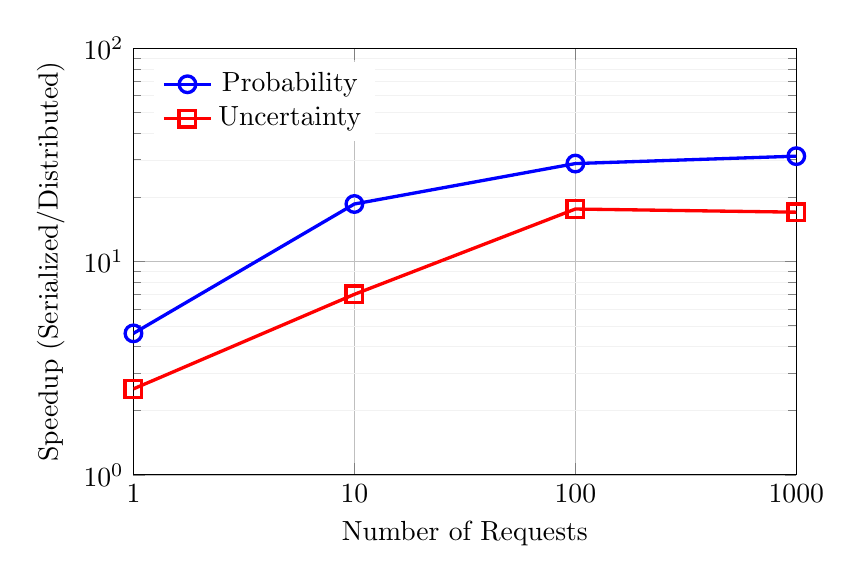
\begin{tikzpicture}
        \begin{loglogaxis}[
            width=10cm,
            height=7cm,
            grid=both,
            minor grid style={line width=.1pt, draw=gray!10},
            major grid style={line width=.2pt, draw=gray!50},
            xlabel={Number of Requests},
            ylabel={Speedup (Serialized/Distributed)},
            legend pos=north west,
            legend style={draw=none},
            xtick={1,10,100,1000},
            xticklabels={1,10,100,1000},
            log basis x=10,
            log basis y=10,
            ymin=1, ymax=100,
            xmin=1, xmax=1000
            ]
            
            % Probability speedup data
            \addplot[
                color=blue,
                mark=o,
                line width=1.2pt,
                mark size=3pt
                ] coordinates {
                (1, 4.603)
                (10, 18.6)
                (100, 28.776)
                (1000, 31.167)
            };
            
            % Uncertainty speedup data
            \addplot[
                color=red,
                mark=square,
                line width=1.2pt,
                mark size=3pt
                ] coordinates {
                (1, 2.528)
                (10, 7.016)
                (100, 17.616)
                (1000, 17.029)
            };
            
            \legend{Probability, Uncertainty}
        \end{loglogaxis}
    \end{tikzpicture}
    \caption{Speedup comparison between serialized and distributed execution for different request volumes.}
    \label{fig:speedup}
\end{figure}